\documentclass[11pt]{article}
 
\usepackage[margin=.95in]{geometry} 
\usepackage{amsmath,amsthm,amssymb, graphicx, multicol, array}
 
\newcommand{\N}{\mathbb{N}}
\newcommand{\Z}{\mathbb{Z}}
 

\begin{document}
 
\title{Homework 1}
\author{Juliette Franqueville\\
}
\maketitle

\subsection*{(1)  For $y_1,.., y_n \sim \mathcal{N}(\mu,\sigma^2 )$, show that $s = (\bar{y},s^2 )$ are sufficient. Also, find the observed and the expected information matrices}

The factorization theorem says that statistic $s$ is sufficient iif $f(y_{1:n}|\theta) = g(s|\theta)h(y_{1:n})$. For the normal, we have:

\begin{align*}
   f(y_{1:n}|\theta) &= \prod (2\pi \sigma^2)^{-1/2} \text{exp}\left(-\frac{(y_i-\mu)^2}{2\sigma^2}\right) \\
   &=(2\pi \sigma^2)^{-n/2}\text{exp}\left(-\frac{\sum (y_i-\mu)^2}{2\sigma^2}\right) \\
    &=(2\pi \sigma^2)^{-n/2}\text{exp}\left(-\frac{\sum ([y_i-\bar{y}]-[\mu-\bar{y})]^2}{2\sigma^2}\right) \\
    &=(2\pi \sigma^2)^{-n/2}\text{exp}\left(-\frac{\sum \{ [y_i-\bar{y}]^2-2[y_i-\bar{y}][\mu-\bar{y}]+[\mu-\bar{y}]^2 \}}{2\sigma^2}\right) \\
        &=(2\pi \sigma^2)^{-n/2}\text{exp}\left(-\frac{\sum \{ [y_i-\bar{y}]^2+[\mu-\bar{y}]^2 \}}{2\sigma^2}\right) \\
        &=(2\pi \sigma^2)^{-n/2}\text{exp}\left(-\frac{\sum  [y_i-\bar{y}]^2}{2\sigma^2}\right) \text{exp}\left(-\frac{n [\mu-\bar{y}]^2}{2\sigma^2}\right) \\
        &=(2\pi \sigma^2)^{-n/2}\text{exp}\left(-\frac{\sum  [y_i-\bar{y}]^2}{2\sigma^2}\right) \text{exp}\left(-\frac{n [\mu-\bar{y}]^2}{2\sigma^2}\right) \\
    &=(2\pi \sigma^2)^{-n/2}\text{exp}\left(-\frac{(n-1)s^2}{2\sigma^2}\right) \text{exp}\left(-\frac{n [\mu-\bar{y}]^2}{2\sigma^2}\right) \\
\end{align*}


We recognize $h(y_{1:n}) =1 $ and $g(\bar{y}, s^2|\mu, \sigma^2)= (2\pi \sigma^2)^{-n/2}\text{exp}\left(-\frac{(n-1)s^2}{2\sigma^2}\right) \text{exp}\left(-\frac{n [\mu-\bar{y}]^2}{2\sigma^2}\right)$ is a sufficient statistic for $(\mu, \sigma^2)$.


\subsection*{(3)  (a) Draw a random sample of size $n = 2$0 from a $\text{Cauchy}(0,1)$ distribution. Compute $\bar{y}n$. Repeat this $B = 1000$ times. Draw a histogram of the sampled $\bar{y}n$ values, superimposed over a $\text{Cauchy(0,1)}$ density.}

\begin{figure}[!h]
    \centering
    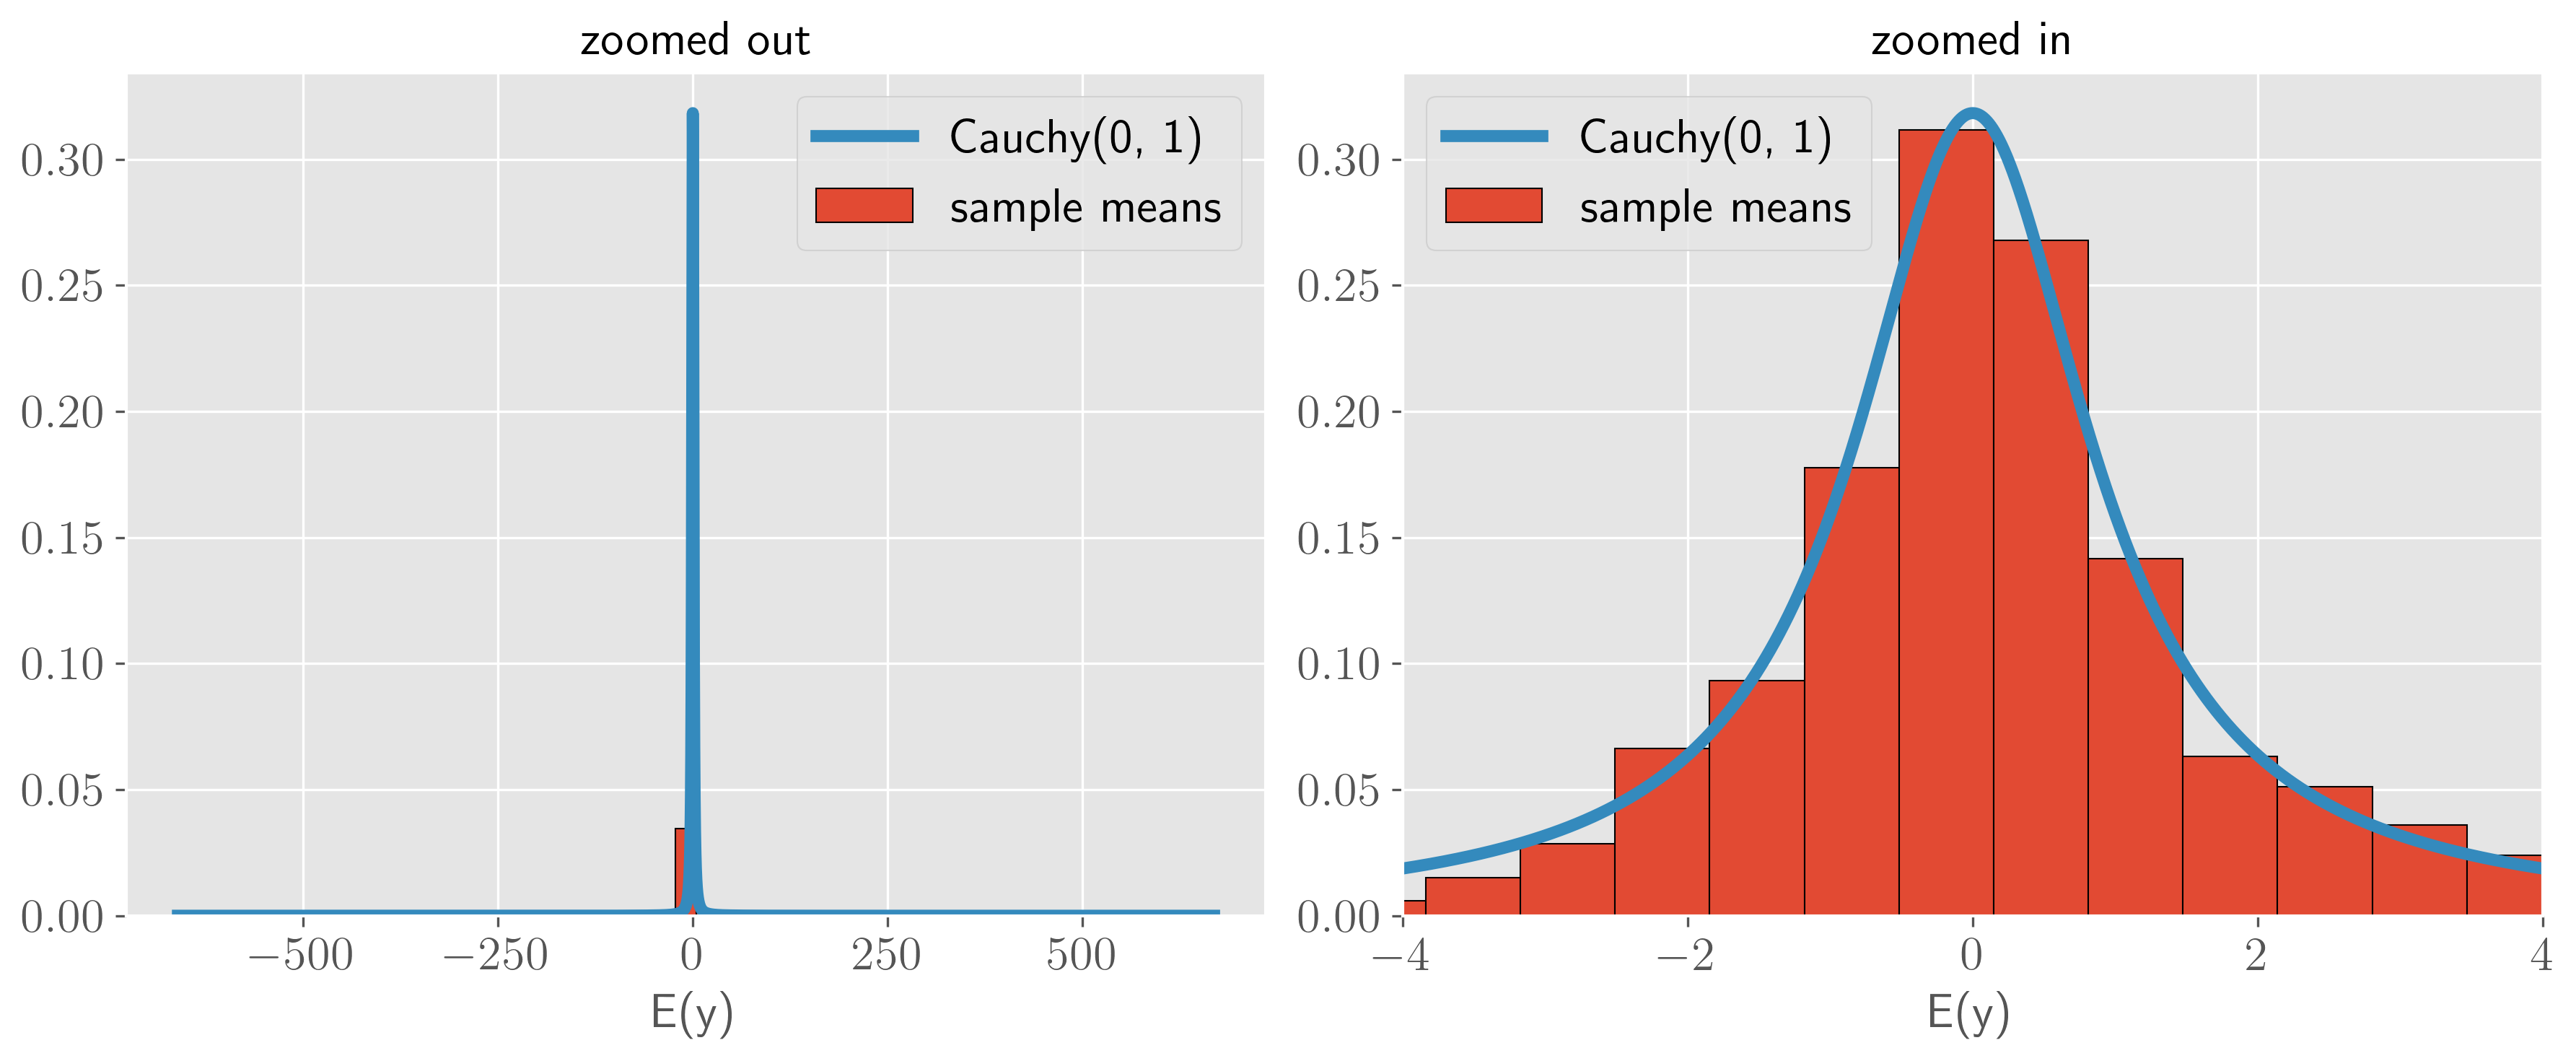
\includegraphics[scale=.55]{homework_2/figures/cauchy_mean.png}
    \caption{Histogram for question (3) (a)}
    \label{fig:my_label}
\end{figure}

\subsection*{Estimate $\theta$ in Cauchy$(\theta, 1)$ using (b) step-wise gradient ascent, (c) Newton-Raphson, and (d) stochastic gradient ascent. }

We need the first and second derivatives of the log likelihood to implement gradient ascent / Newton-Raphson / tochastic gradient ascent. 

\begin{align*} log L(\theta) &= log \prod_{i=1}^n \frac{1}{\pi}\frac{1}{1+(y_i-\theta)^2} \\
&= \sum_{i=1}^n log \frac{1}{\pi}\frac{1}{1+(y_i-\theta)^2} \end{align*}
\begin{align*} \frac{d}{d\theta}log L(\theta) &= \frac{d}{d\theta}\sum_{i=1}^n log \frac{1}{\pi}\frac{1}{1+(y_i-\theta)^2} \\
&=  \sum_{i=1}^n   \frac{2(y_i-\theta)}{1+(y_i-\theta)^2}\end{align*}

\begin{align*} H(\theta) &=\sum_{i=1}^n   \frac{2(y_i-\theta)}{1+(y_i-\theta)^2} \\
&=  \sum_{i=1}^n   \frac{2[(y_i-\theta)^2-1]}{[1+(y_i-\theta)^2]^2} \end{align*}

For gradient ascent and stochastic gradient ascent, we have:

\begin{align*}
    \theta^{(m+1)} = \theta^{(m)} + \gamma \frac{\partial \mathcal{L}(\theta^{(m)})}{\partial \theta}
\end{align*}

For stochastic gradient ascent, we randomly choose a single sample to evaluate the log likelihood at each iteration. For Newton-Raphson (this is the general multidimensional form, we only have one unknown here):

\begin{align*}
    \theta^{(m+1)} = \theta^{(m)} - H(\theta^{(m)})^{-1} \frac{\partial \mathcal{L}(\theta^{(m)})}{\partial \theta}
\end{align*}

Note that the log likelihood was not strictly concave (its second derivative is not strictly negative). Therefore, the optimizations were repeated several times at different starting values and the run resulting in the highest MLE was chosen. The scripts are attached to this homework.

\begin{figure}[!h]
    \centering
    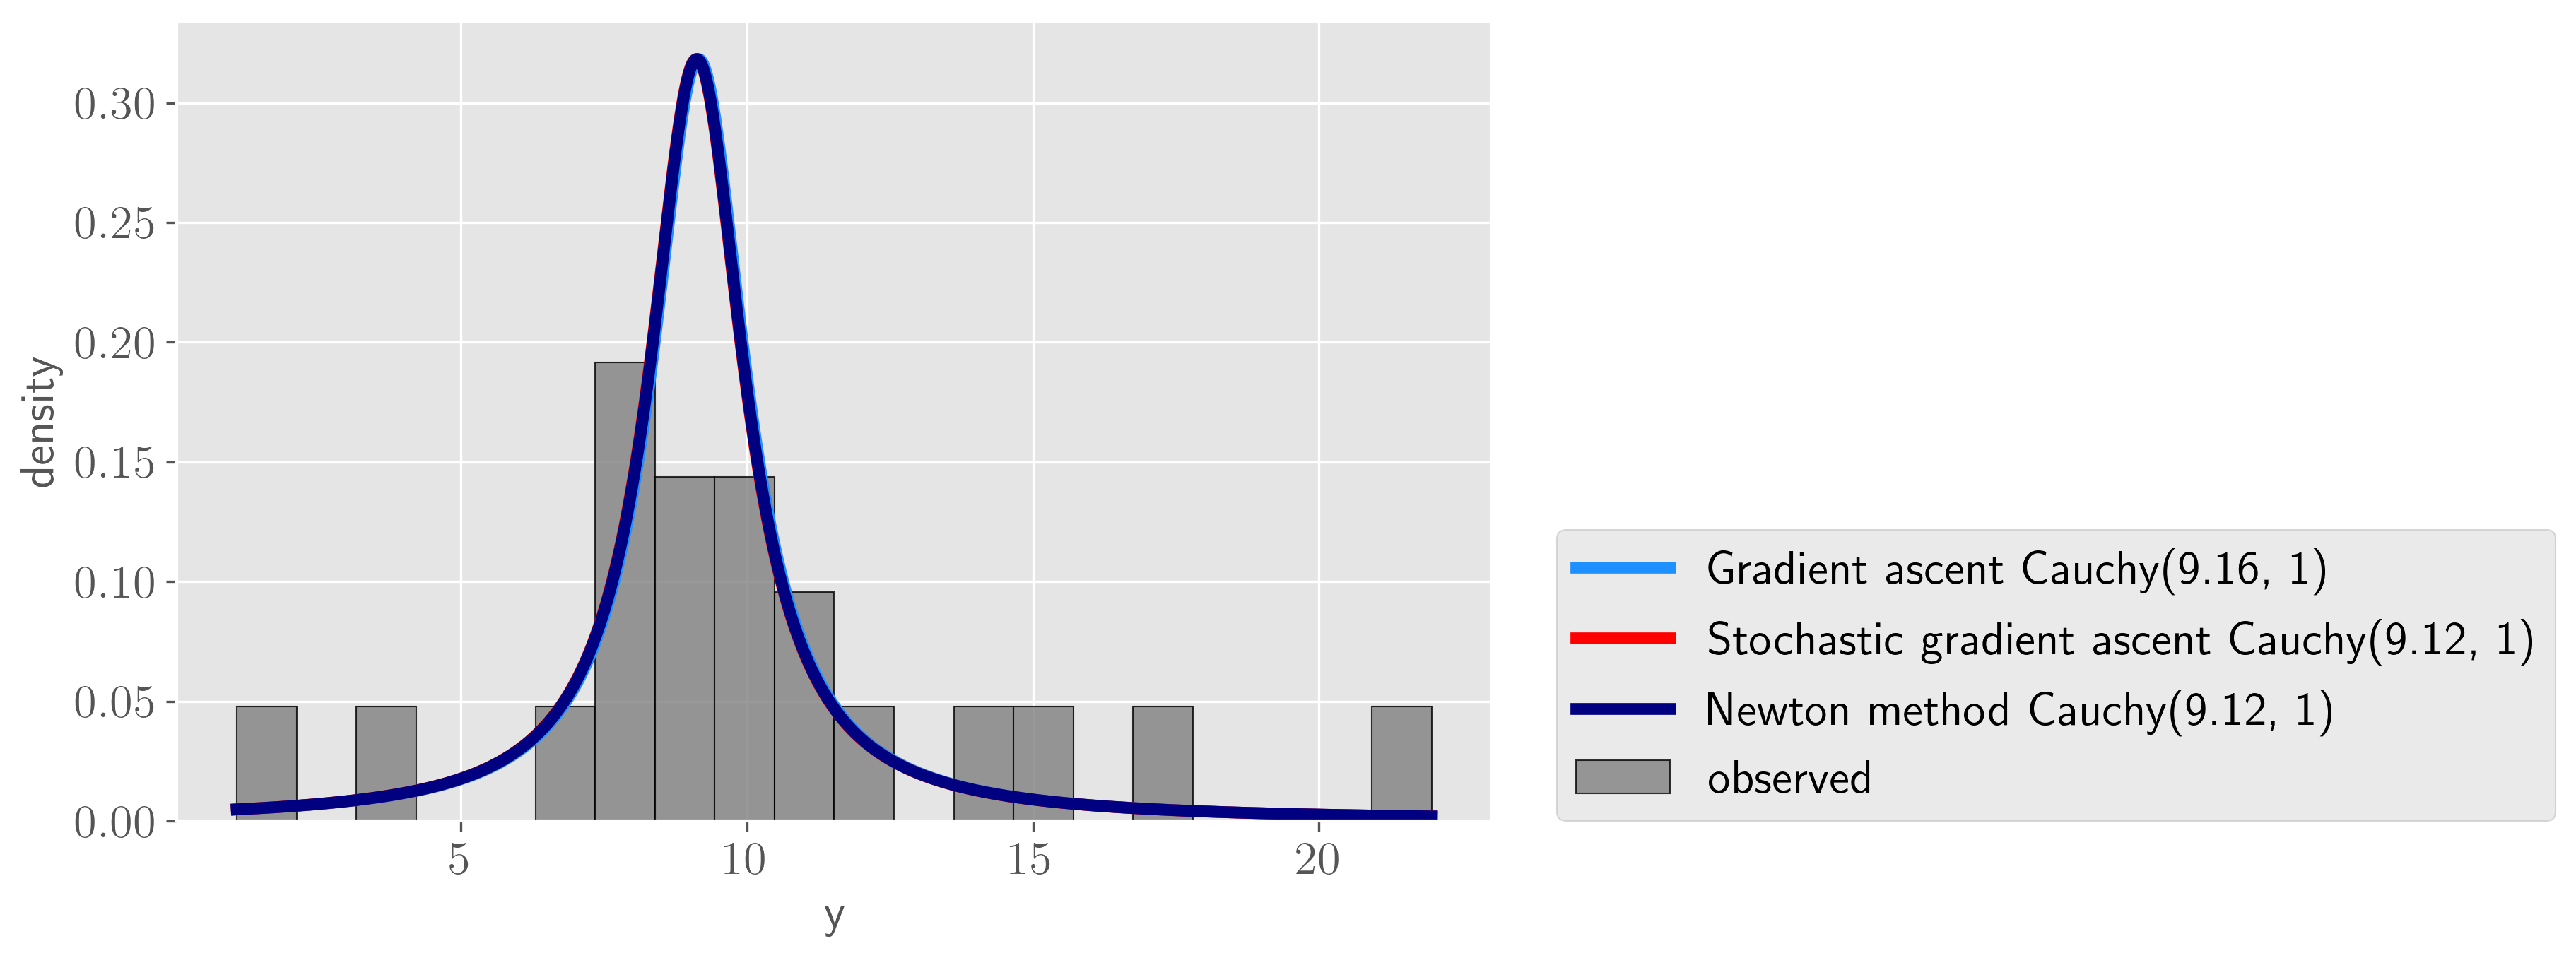
\includegraphics[scale=.55]{homework_2/figures/mle_cauchy.png}
    \caption{Cauchy($\theta$, 1) for the three methods using their $\theta_{MLE}$}
    \label{fig:my_label}
\end{figure}

\begin{figure}[!h]
    \centering
    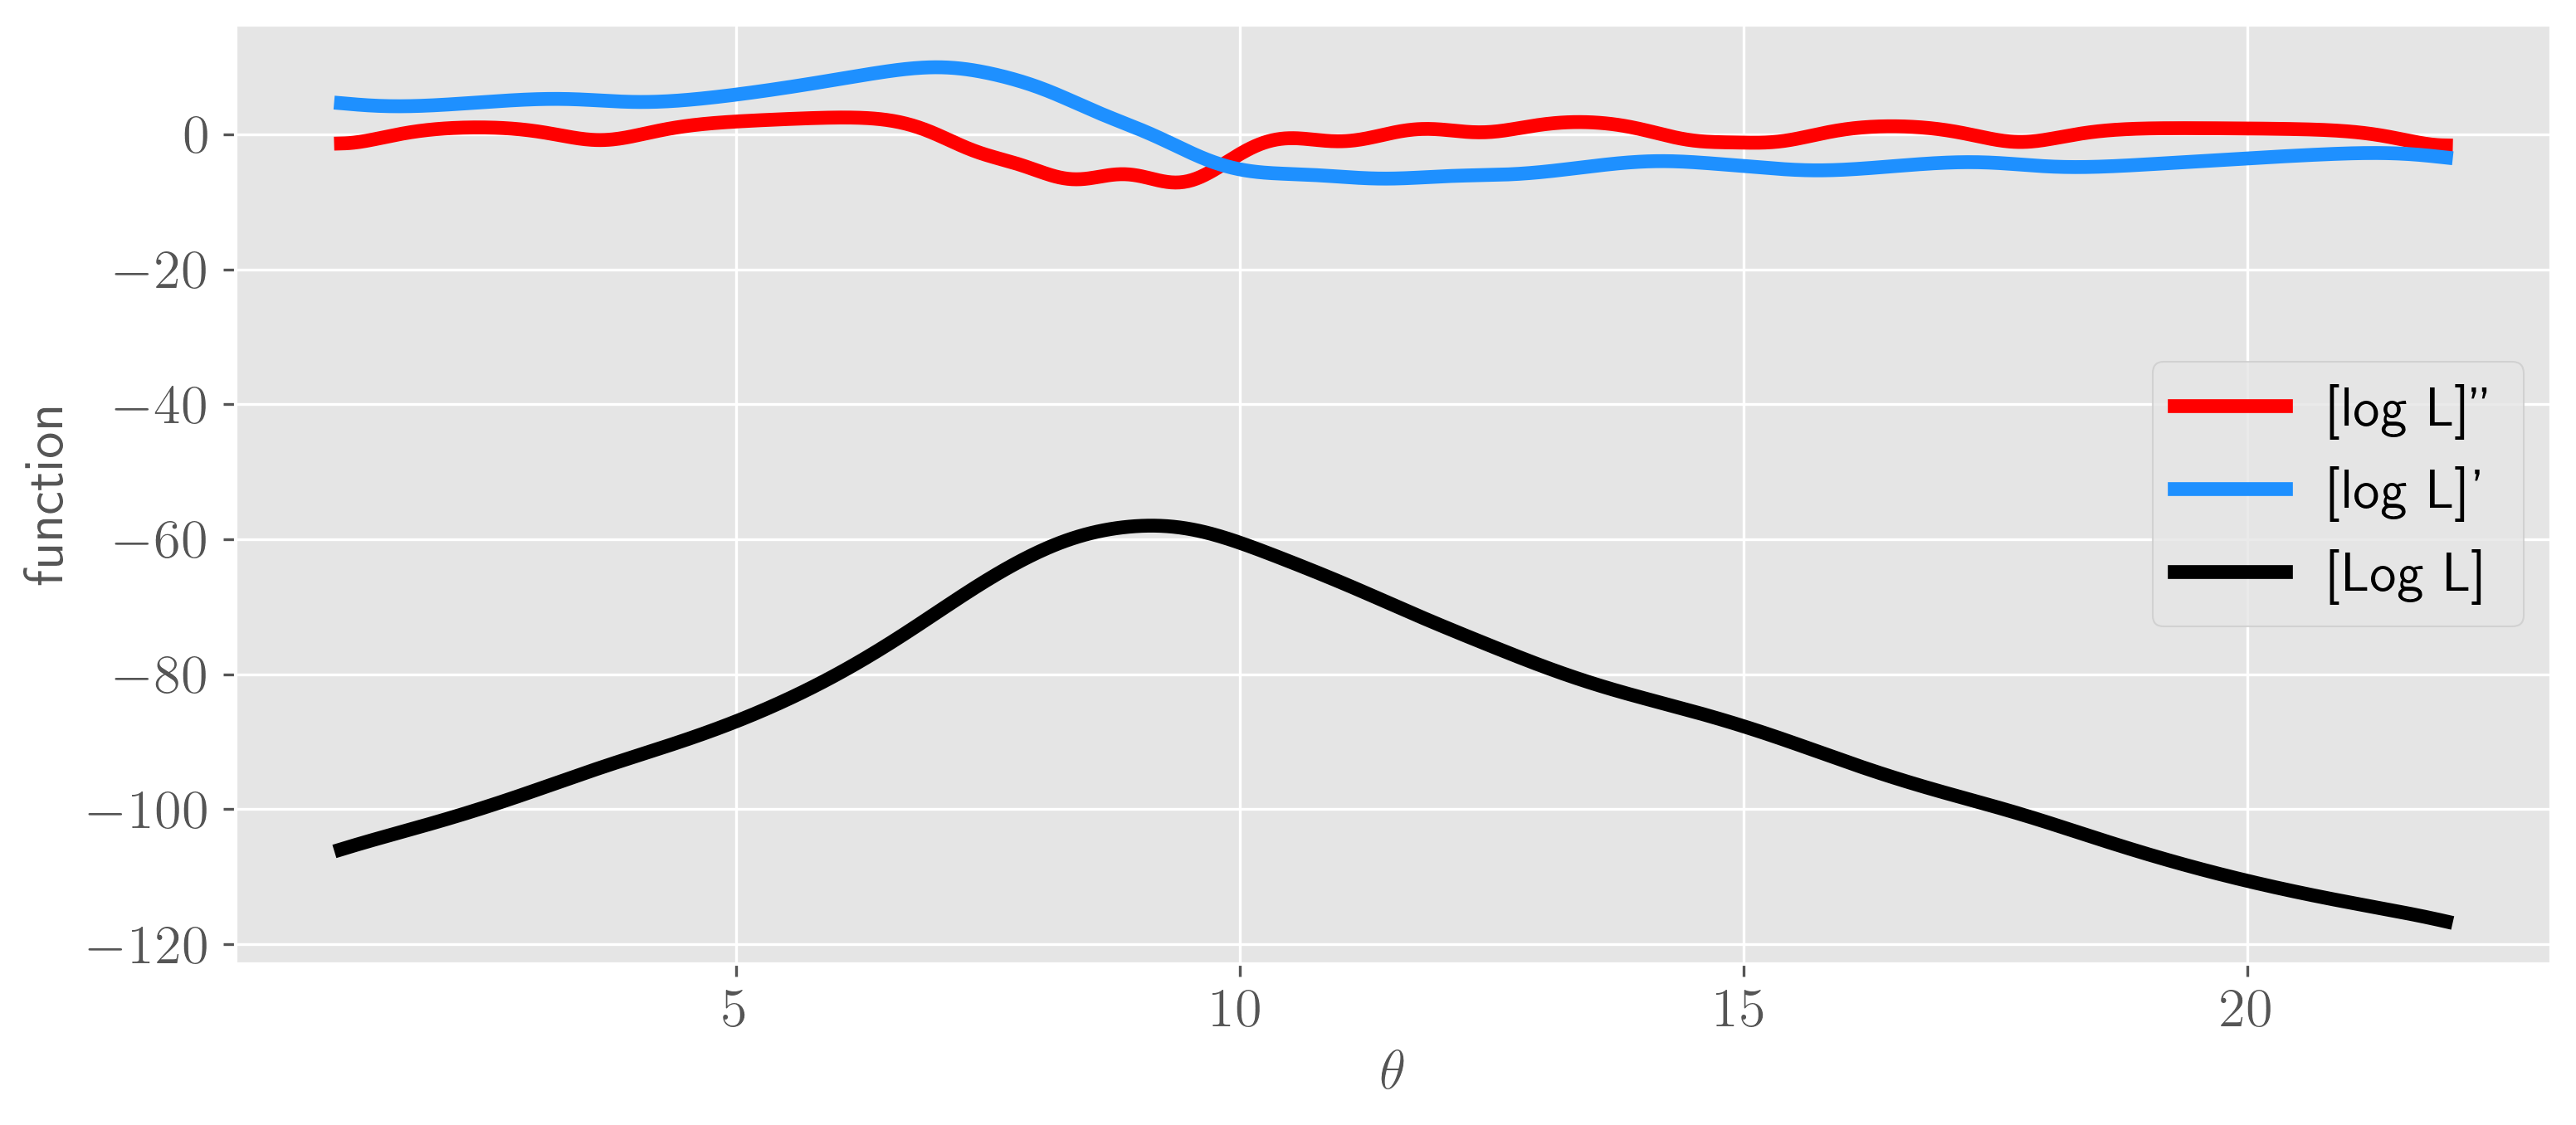
\includegraphics[scale=.55]{homework_2/figures/cauchy_fns.png}
    \caption{Log likelihood and its first and second derivatives}
    \label{fig:my_label}
\end{figure}

\begin{figure}[!h]
    \centering
    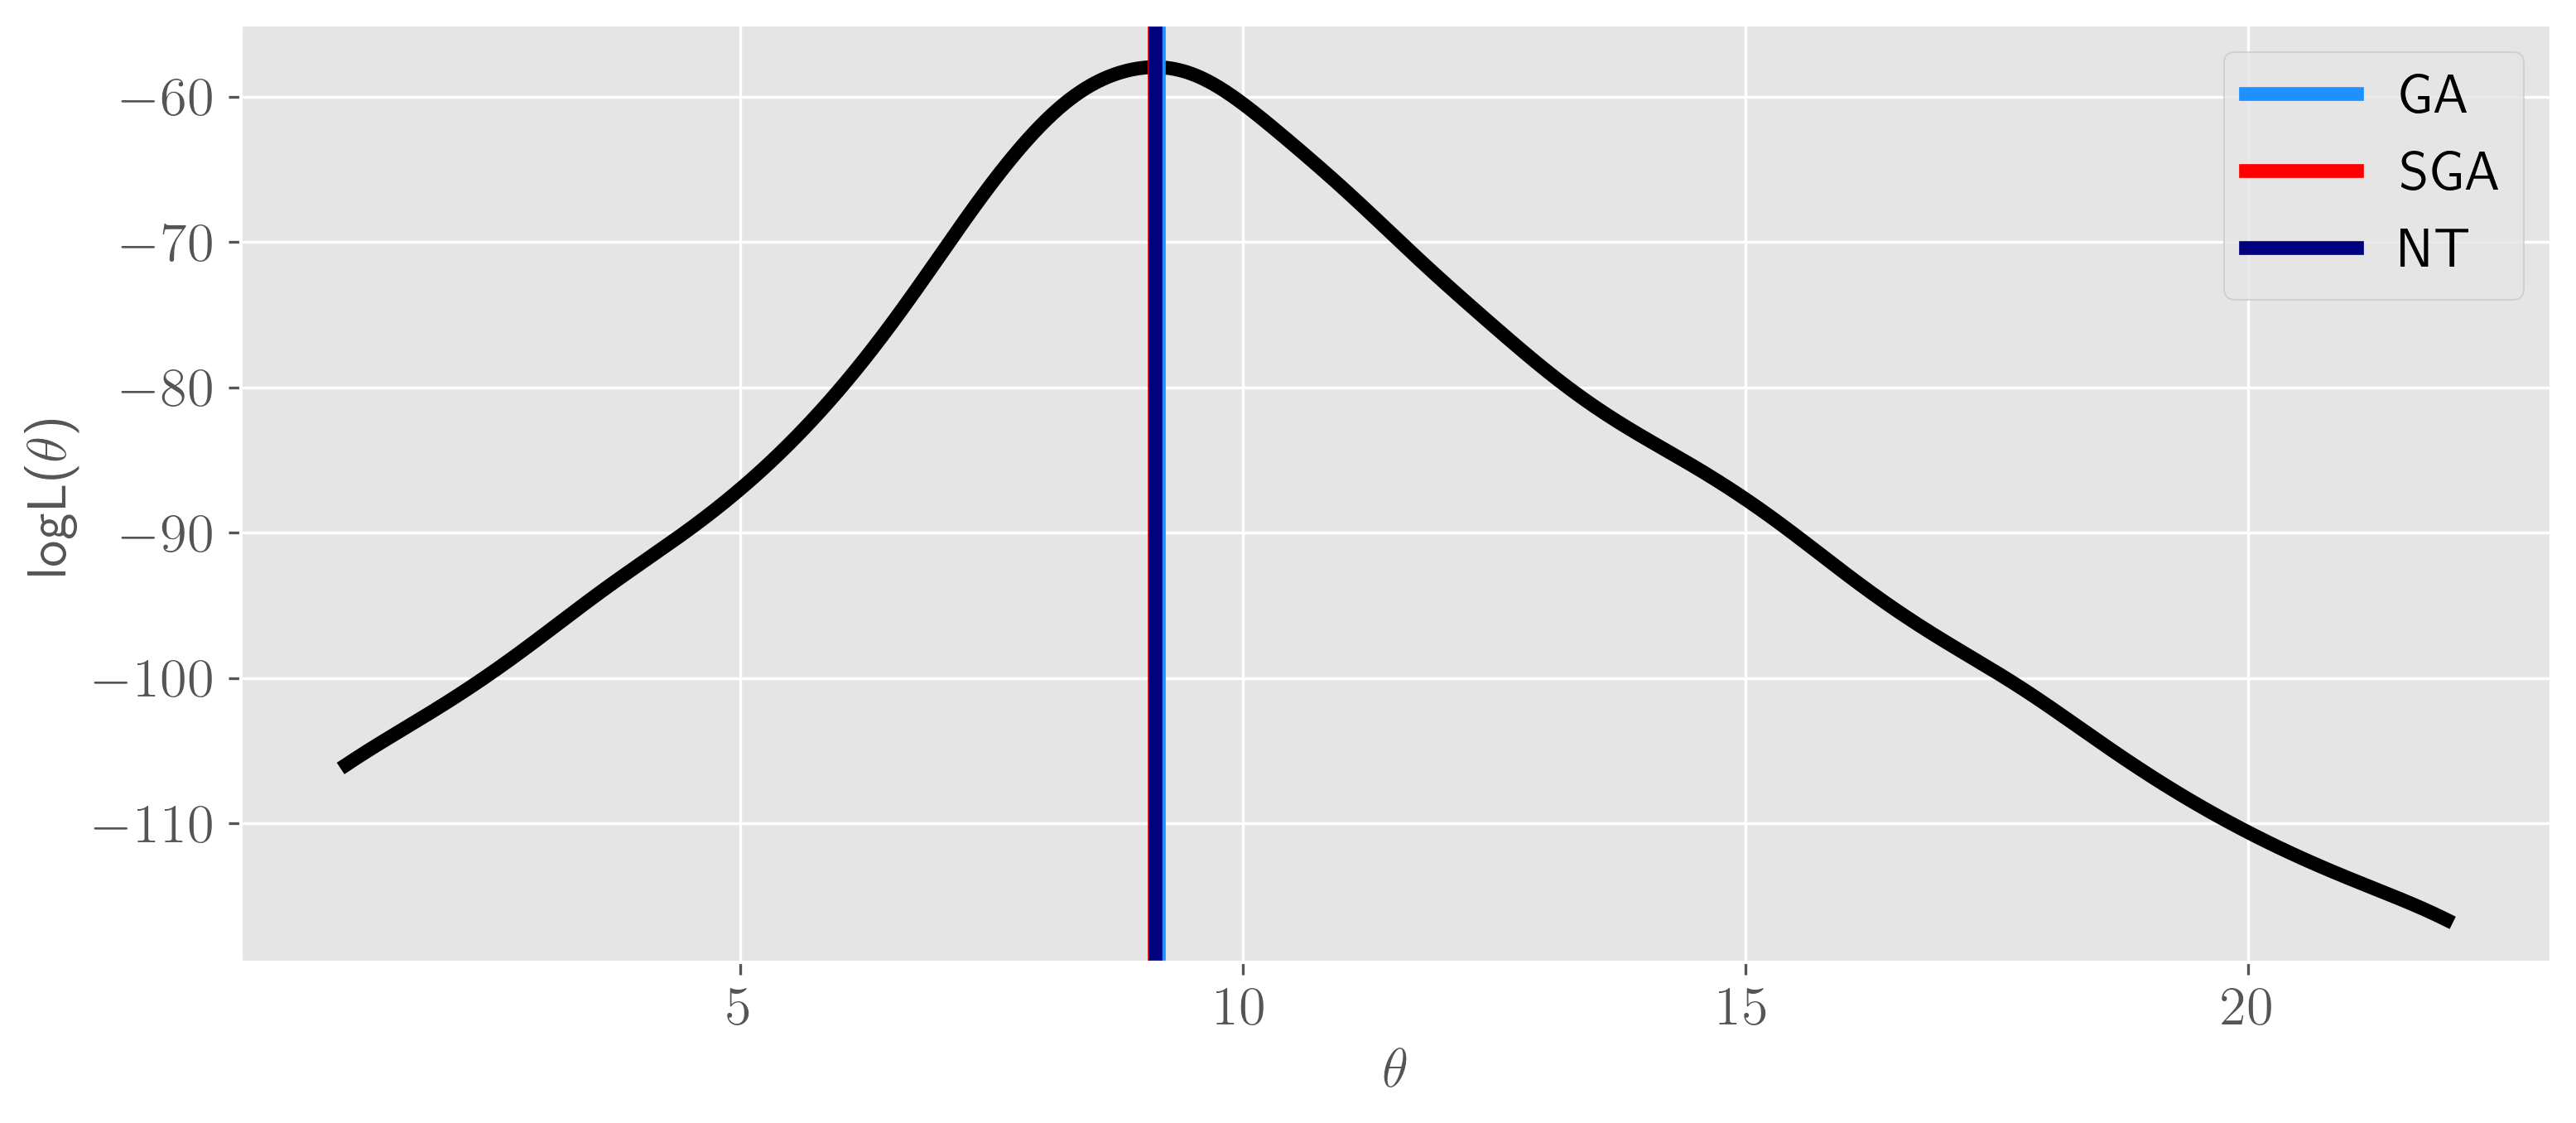
\includegraphics[scale=.55]{homework_2/figures/cauchy_loglike.png}
    \caption{Log likelihood and the $\theta$ values for the three optimizers (they overlap).}
    \label{fig:my_label}
\end{figure}

Newton-Raphson converged in 3 iterations (given the tolerance specified). The two other algorithms took larger number of iterations. In terms of time, Newton-Raphson was also the fastest algorithm to converge.

\subsection*{(4) Let $y_{i,j}$
ind∼ $Normal(\mu_i,\sigma^2)$, $i = 1,...,n$ and $j = 1,...,m$ with $n \xrightarrow[]{} \infty$
but m fixed. Find out the MLEs of $\mu_i$ and $\sigma^2$. Show that  $\hat{\sigma}^2$ MLE is inconsistent for $\sigma^2$. Adjust this estimator to come up with a consistent estimator of  $\sigma^2$.}

We have

\begin{align*}
    L(\mu, \sigma^2) &=  (2\pi \sigma^2)^{-n/2} \text{exp} \left(- \frac{\sum(y_i-\mu)^2}{2\sigma^2}\right)\\
    \mathcal{L}(\mu, \sigma^2) &= -\frac{n}{2}log(2\pi)  -\frac{n}{2}log(\sigma^2)  -\frac{1}{2\sigma^2}\sum(y_i-\mu)^2
\end{align*}

and 

\begin{align*}
    \frac{\partial \mathcal{L}(\mu, \sigma^2)}{\partial \mu} &= 0 \\
    -\frac{1}{2\sigma^2} \sum -2(y_i-\mu)&= 0 \\
     \sum y_i-n\mu&= 0 \\
     \sum \mu&= \bar{y} \\
\end{align*}

\begin{align*}
    \frac{\partial \mathcal{L}(\mu, \sigma^2)}{\partial \sigma^2} &= 0 \\
    -\frac{n}{2\sigma^2} + \frac{1}{2\sigma^4}\sum (y_i - \mu)^2&= 0 \\
     -\frac{n}{2} + \frac{1}{2\sigma^2}\sum (y_i - \mu)^2&= 0 \\
     -\sigma^2n +\sum (y_i - \mu)^2&= 0 \\
     \sigma^2 &= \sum (y_i - \mu)^2 / n \\
\end{align*}

In practice we would replace $\mu$ with $\bar{y}$. But

\begin{align*}
    E(\sigma^2_{MLE}) &= E\left(\sum (y_i - \bar{y})^2 / n\right)\\
    &= \frac{1}{n} E\left(\sum y_i^2 - 2\bar{y} \sum y_i + \bar{y}n \right)\\
    &= \frac{1}{n} E\left( y_i^2 - 2\bar{y}^2n + \bar{y}^2n \right)\\
     &= \frac{1}{n} E\left( \sum y_i^2 - \bar{y}^2n \right)\\
      &= \frac{1}{n} E\left( \sum y_i^2 - \bar{y}^2n \right)\\
       &=  E( y^2) - E(\bar{y}^2)\\
          &=  var(y) + E(y)^2 - var(\bar{y}) - E(\bar{y})^2 \\
            &=  var(y)  - var(\bar{y}) \\
              &=  var(y)  - var(y)/n \\
               &=  \frac{(n-1)\sigma^2}{n}\\
\end{align*}
So, a better estimator is $\sum (y_i - \mu)^2 / (n-1) $.

\subsection*{(5) For $y_1,...,y_n \sim Uniform(0, 
\theta)$, show that $ z_n = \frac{n(\theta-\hat{\theta}_{MLE})}{\theta} \xrightarrow[]{D} E$, where E is exponential. Design a simulation study illustrating this nice result.}

We have, for $y \in [0, \theta]$

\begin{align*}
    f(y) &= 1/\theta \\ 
    L(\theta) &= 1/ \theta ^n\\
\end{align*}

In order to maximize $L(\theta)$, it is obvious that $\theta = max(y_i)$ because if it is less than $ max(y_i)$, samples will be left out (which  will have probability 0).

\begin{align*}
    P\left(\frac{n[\theta-\hat{\theta}_{MLE}] }{\theta} \leq t\right) &= 1 -  P\left(\frac{n[\theta-\hat{\theta}_{MLE}] }{\theta}  \geq t\right)\\
    &= 1 -  P\left(\hat{\theta}_{MLE}  \leq \frac{\theta[t-n]}{n} \right)\\
     &= 1 -  P\left(\hat{\theta}_{MLE}  \leq \frac{\theta[t-n]}{n} \right)\\
      &= 1 -  P\left(max(y)  \leq \frac{\theta[t-n]}{n} \right)\\
       &= 1 -  \prod P\left(y_i  \leq \frac{\theta[t-n]}{n} \right)\\
        &= 1 -  \left( \frac{\frac{\theta[t-n]}{n}}{\theta} \right)^n\\
          &= 1 -  (1-t/n)^n\\
\end{align*}

and $\lim_{n\to\infty}  1 -  (1-t/n)^n = 1-\text{exp}(-t)$, which is the cdf of $\exp(1)$. So we have shown that $ z_n = \frac{n(\theta-\hat{\theta}_{MLE})}{\theta} \xrightarrow[]{D} E$, where E is exponential. This result is illustrated in the plot below.

\end{document}